\section{Анализ предметной области}
\subsection{Понятие распознавания лица}

Распознавание лиц — это технология, позволяющая идентифицировать или верифицировать личность человека на основе изображения, видеозаписи или других визуальных данных, связанных с лицом. Несмотря на разнообразие технических решений, все системы распознавания лиц стремятся к одной цели — точному сопоставлению биометрических данных с конкретным человеком из базы.\cite{sis}

Процесс распознавания можно разделить на четыре основных этапа:

\begin{enumerate}
	\item Обнаружение лица.
	\item Определение ключевых точек лица.
	\item Преобразование в цифровой вид.
	\item Сопоставление с базой данных.
\end{enumerate}

\subsection{История развития систем распознавания лица}

Первые научные исследования в области автоматического распознавания лиц были начаты в 1960-х годах. На этом первоначальном этапе процесс автоматизации был реализован лишь частично: человек вручную отмечал ключевые точки лица. Это были центры зрачков, уголки глаз, средняя точка на линии роста волос в верхней части лба и другие. Для этих точек затем вычислялся набор из 20 взаимных расстояний, которые и служили формальным описанием лица.

Такая полуавтоматическая система демонстрировала производительность на уровне до 40 распознанных лиц в час, причем основным ограничивающим фактором выступала скорость работы человека, ответственного за корректную расстановку ключевых точек. Несмотря на низкую производительность по современным меркам, подобные системы отлично подходили для задач идентификации преступников по фотографиям, где требования к скорости обработки были существенно ниже, чем в реальном времени.

В 1970-х годах были предприняты первые попытки полной автоматизации процесса расстановки ключевых точек, однако достигнутые результаты не отличались достаточной надежностью.

В 1987 г. был предложен подход, основанный на представлении изображения лица собственными векторами, полученными из матрицы изображения. Подход получил название eigenface. В основе этого подхода лежало представление черно-белого изображения лица в виде матрицы яркостей пикселей. После центрирования данных путем вычитания среднего значения яркости, матрица преобразовывалась в вектор, для которого строилась матрица ковариаций. Для этой матрицы вычислялся собственный вектор (eigenvectors), причем несколько наибольших по модулю компонент такого вектора использовались в качестве компактного описания лица. Хотя данный алгоритм изначально не был специфически разработан для задач распознавания лиц, а представлял собой общий метод анализа образов, он заложил важные основы для последующего развития более специализированных алгоритмов. В дальнейшем этот подход был адаптирован для выделения и анализа отдельных частей лица: глаз, носа и рта.

В 1990-х годах специально для решения задачи распознавания лиц были собраны первые крупномасштабные базы данных лиц. Эти базы данных содержали тысячи изображений, сделанных в различных условиях освещения и с небольшими вариациями наклона головы. В отличие от ранее использовавшихся фотографий преступников, сделанных в стандартизированных условиях после задержания, новые базы данных позволяли более объективно оценивать качество алгоритмов распознавания. Например, база данных FERET включала более 14 000 изображений 1 200 различных людей и стала стандартным инструментом для сравнительного анализа методов распознавания. В 1990-х годах системы автоматического распознавания лиц начали находить первое коммерческое применение.

В 2001 г. появился быстрый алгоритм для решений задачи детекции –  метод Виолы-Джонса  Этот метод основывался на использовании интегрального представления изображения, где значение каждого пикселя вычислялось как сумма значений всех пикселей, расположенных левее и выше данного.

Алгоритм применял скользящее окно, которое последовательно проходило по всему изображению с заданным шагом, вычисляя разность сумм пикселей внутри черных и белых областей специальных карт признаков (рис ~\ref{fig:haar}). Каждая такая карта признаков кодировала определенные характеристики частей лица. Процесс сканирования повторялся многократно с различными размерами окна и разными наборами карт признаков, что позволяло получить комплексное описание изображения в виде набора признаков Хаара.

Для повышения эффективности в алгоритме Виолы-Джонса использовался каскадный принцип вычислений: если на начальных этапах обработки определенной области изображения не обнаруживалось достаточного количества соответствий, дальнейшие вычисления для этой области прекращались. Благодаря такой оптимизации метод достиг высокой скорости работы и получил широкое распространение, в частности, в цифровых фотоаппаратах для реализации функции автоматического обнаружения лиц.

Однако этот подход имел и существенные ограничения: он мог надежно детектировать только фронтальные изображения лиц с наклоном не более 30 градусов и был подвержен относительно высокому уровню ложных срабатываний.
\begin{figure}[H]
	\centering
	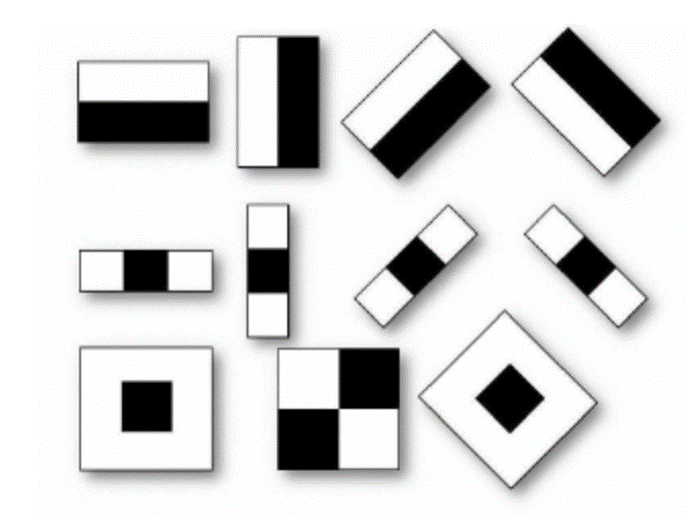
\includegraphics[width=0.7\linewidth]{images/Haar}
	\caption{Карта признаков Хаара}
	\label{fig:haar}
\end{figure}
\begin{figure}[H]
	\centering
	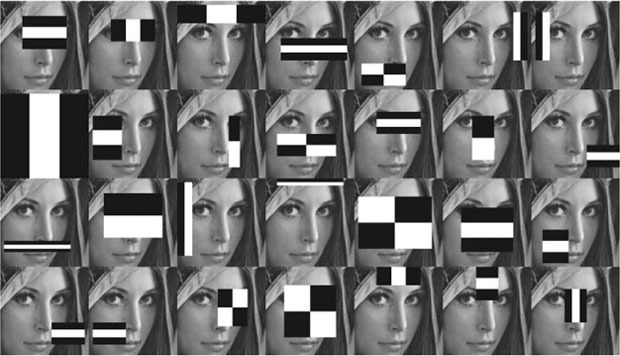
\includegraphics[width=0.7\linewidth]{images/haar2}
	\caption{Пример детекции частей лица картами признаков Хаара}
	\label{fig:haar2}
\end{figure}

С начала 2000-x гг. для распознавания лиц используется метод опорных векторов, скрытые марковские модели и начинают использоваться простые свёрточные нейронные сети.

В этот же период появились новые масштабные коллекции изображений лиц, такие как Labeled Faces in the Wild (LFW), содержащие 13 000 изображений 1 680 различных людей, сделанных в естественных условиях с вариациями освещения, выдержки и поз.

В 2007 году был предложен комбинированный подход, сочетающий локальные бинарные шаблоны (LBP) и фильтры Габора. LBP-преобразование эффективно сохраняло информацию о мелких деталях изображения, в то время как фильтры Габора обеспечивали инвариантность к масштабу и сохраняли информацию о общей форме лица. На заключительном этапе применялся метод главных компонент (PCA) для получения компактного описания лица.

Вместе с рядом прорывов в задачах классификации изображений (2012 г. –  AlexNet) заметно улучшаются и системы распознавания лиц. Рост вычислительных мощностей, включая широкое использование GPU, сделал возможным обучение глубоких нейронных сетей, в частности свёрточных нейронных сетей (CNN).

Важным преимуществом CNN стало то, что они автоматически обучались оптимальным фильтрам для выделения значимых признаков, избавляя разработчиков от необходимости ручного подбора характеристик. Нейроны в различных слоях сети специализировались на распознавании признаков разного уровня абстракции: от простых геометрических примитивов (линий, углов) на начальных слоях до сложных семантических признаков (глаза, нос, рот) на глубоких слоях.

В 2014 году система DeepFace продемонстрировала точность распознавания 97\% на базе данных LFW, впервые достигнув человеческого уровня.

Современные системы на основе глубокого обучения, такие как FaceNet и ArcFace, демонстрируют точность выше 99.9\% на стандартных тестовых наборах данных. Они обладают устойчивостью к изменениям освещения, ракурса и частичным перекрытиям лица.\cite{history}

\subsection{Выбор метода распознавания лица}

Существует множество методов распознавания лиц, различающихся по точности, скорости, устойчивости к внешним условиям и требованиям к ресурсам. Наиболее популярными являются следующие подходы: алгоритм Виолы-Джонса (Haar Cascades), метод гистограмм направленных градиентов (HOG) и многозадачная сверточная нейронная сеть (MTCNN).\cite{four}

\subsubsection{Алгоритм Виолы-Джонса (Haar Cascades)}
Алгоритм Виолы-Джонса — это один из первых и наиболее известных методов обнаружения объектов на изображениях в реальном времени, особенно лиц. Он был представлен Полом Виолой и Майклом Джонсом в 2001 году и до сих пор используется в различных приложениях компьютерного зрения благодаря своей эффективности и скорости. Он основан на использовании простых признаков — так называемых признаков Хаара, напоминающих вейвлет-фильтры. Метод последовательно применяет каскад классификаторов, обученных с использованием алгоритма AdaBoost. Каждый этап каскада фильтрует изображения, уменьшая количество проверяемых областей.

Основное преимущество алгоритма — высокая скорость распознавания при малом потреблении ресурсов. Однако метод чувствителен к изменению условий: освещению, положению головы, мимике, а также плохо работает с тёмным оттенком кожи и при частичном перекрытии лица. Сегодня данный подход используется преимущественно в простых задачах с контролируемыми условиями.

\subsubsection{Гистограмма направленных градиентов (HOG)}
Гистограмма направленных градиентов (Histogram of Oriented Gradients) представляет изображение в виде вектора признаков, отражающего ориентацию градиентов яркости в отдельных ячейках изображения. Эти признаки являются устойчивыми к небольшим изменениям освещения и масштабирования. Далее полученный дескриптор подаётся в классификатор, как правило, линейный метод опорных векторов.

HOG был популярен в системах распознавания пешеходов и других объектов с устойчивыми очертаниями. Однако при распознавании лиц метод показывает невысокую точность. Он плохо справляется с поворотами головы и изменениями выражения лица, поскольку чувствителен к геометрическим искажениям. Кроме того, метод имеет высокую вычислительную сложность: необходимо рассчитать градиенты для каждого пикселя, что замедляет обработку, особенно на слабых устройствах.

\subsubsection{Сверточные нейронные сети и MTCNN}
Современные системы распознавания лиц преимущественно основаны на нейросетевых архитектурах. Одним из таких решений является многозадачная сверточная нейронная сеть — MTCNN (Multi-task Cascaded Convolutional Neural Network). Данный подход объединяет детекцию лиц и определение ключевых точек (глаз, нос, рта) в рамках единой модели. MTCNN состоит из трёх последовательно работающих сетей: P-Net, R-Net и O-Net, каждая из которых уточняет результаты предыдущей.

Главное преимущество MTCNN — высокая точность и устойчивость к различным условиям: поворот головы, частичное перекрытие, различные оттенки кожи и освещения. Метод может эффективно работать даже с деформированными и профильными изображениями лиц. При наличии графического ускорителя (GPU) обработка осуществляется быстро, что делает этот подход оптимальным выбором для реальных систем биометрической идентификации.

\subsection{Проблемы и недостатки современных методов распознавания лица}

Современные системы распознавания лиц на основе искусственного интеллекта могут достигать точности более 95\%, а некоторые системы достигают 99,5\%.\cite{abdulaev} Однако это возможно только в лабораторных или строго управляемых условиях: при хорошем освещении, правильном угле обзора, высоком разрешении камер и минимальных помехах. В реальных условиях эксплуатации — в общественных местах, на улице или в транспорте — точность существенно снижается, а риски ошибок возрастают.

На точность распознавания влияют следующие факторы:
\begin{enumerate}
	\item Освещение и поза. Программы анализа лиц лучше всего работают с изображениями, на которых человек смотрит прямо в камеру. Условия освещения должны быть достаточно яркими, чтобы запечатлеть все черты лица, но не засвечивать их. Положение лица также меняется при повороте головы и зависит от угла обзора наблюдателя. 
	\item Выражения лица. Нейтральное выражение идеально подходит для точного распознавания. Однако наши эмоции и настроение постоянно меняются, как и мимика. Эти различия меняют внешний вид лица, и для систем распознавания становится трудным его идентифицировать.
	\item Старение. Естественные возрастные изменения внешности человека также влияют на способность систем распознавания лиц аутентифицировать людей.
	\item Косметологические вмешательства, смена стиля.  Изменения во внешности благодаря пластическим операциям, макияжу, смене прически могут негативно отразиться на точности срабатывания алгоритмов  распознавания.
	\item Аксессуары. Наличие на лице различных объектов (очки, борода и т.д.) или ношение других аксессуаров, таких как головные уборы, шарфы, может серьезно повлиять на работу системы распознавания. Но современные алгоритмы отрабатывают способность видеть сквозь эти препятствия.\cite{abdulaev}
\end{enumerate}

В условиях, отличных от идеальных, такие системы все ещё способны допускать серьёзные ошибки. За всю историю развития распознавания лиц в России и мире происходило много крупных скандалов, связанных с использованием автоматических систем биометрической идентификации. 

Больше всего скандалов случается, когда системы распознавания лиц путают людей с похожими на них преступниками, вследствие чего людям приходится доказывать свою непричастность перед правоохранительными органами. Один из наиболее известных инцидентов произошёл в Москве, где система распознавания лиц, интегрированная в камеры видеонаблюдения, неверно определила личность прохожего, что привело к его задержанию. Впоследствии выяснилось, что ошибка была вызвана сильным визуальным сходством с разыскиваемым человеком и недостаточной уникальностью биометрических признаков.\cite{moscow} В подобных случаях ошибочное распознавание лиц является неприемлимым, а 5\% ошибок - слишком большим числом.

	